\chapter{Long Term Evolution}
\label{chap:lte}

\section{Digital Communications Overview}
\label{lte:digicomm}

The purpose of a digital communication system is to transport an information
bearing signal from a source to a user destination via a communication channel.
The transmitter, receiver and channel are the three basic elements of a digital
communication system as shown in Figure \ref{fig:digicomsimple}. The message
produced by a source is a digital message, binary and not electrical. An input
transducer is used for converting the message to a time-varying electrical
quantity called waveform. Similarly, at the destination point, another transducer
converts the electrical waveform to the appropriate message.


%esquema básico do sistema de comunicacao
\begin{figure}[htbp]
    \centering
    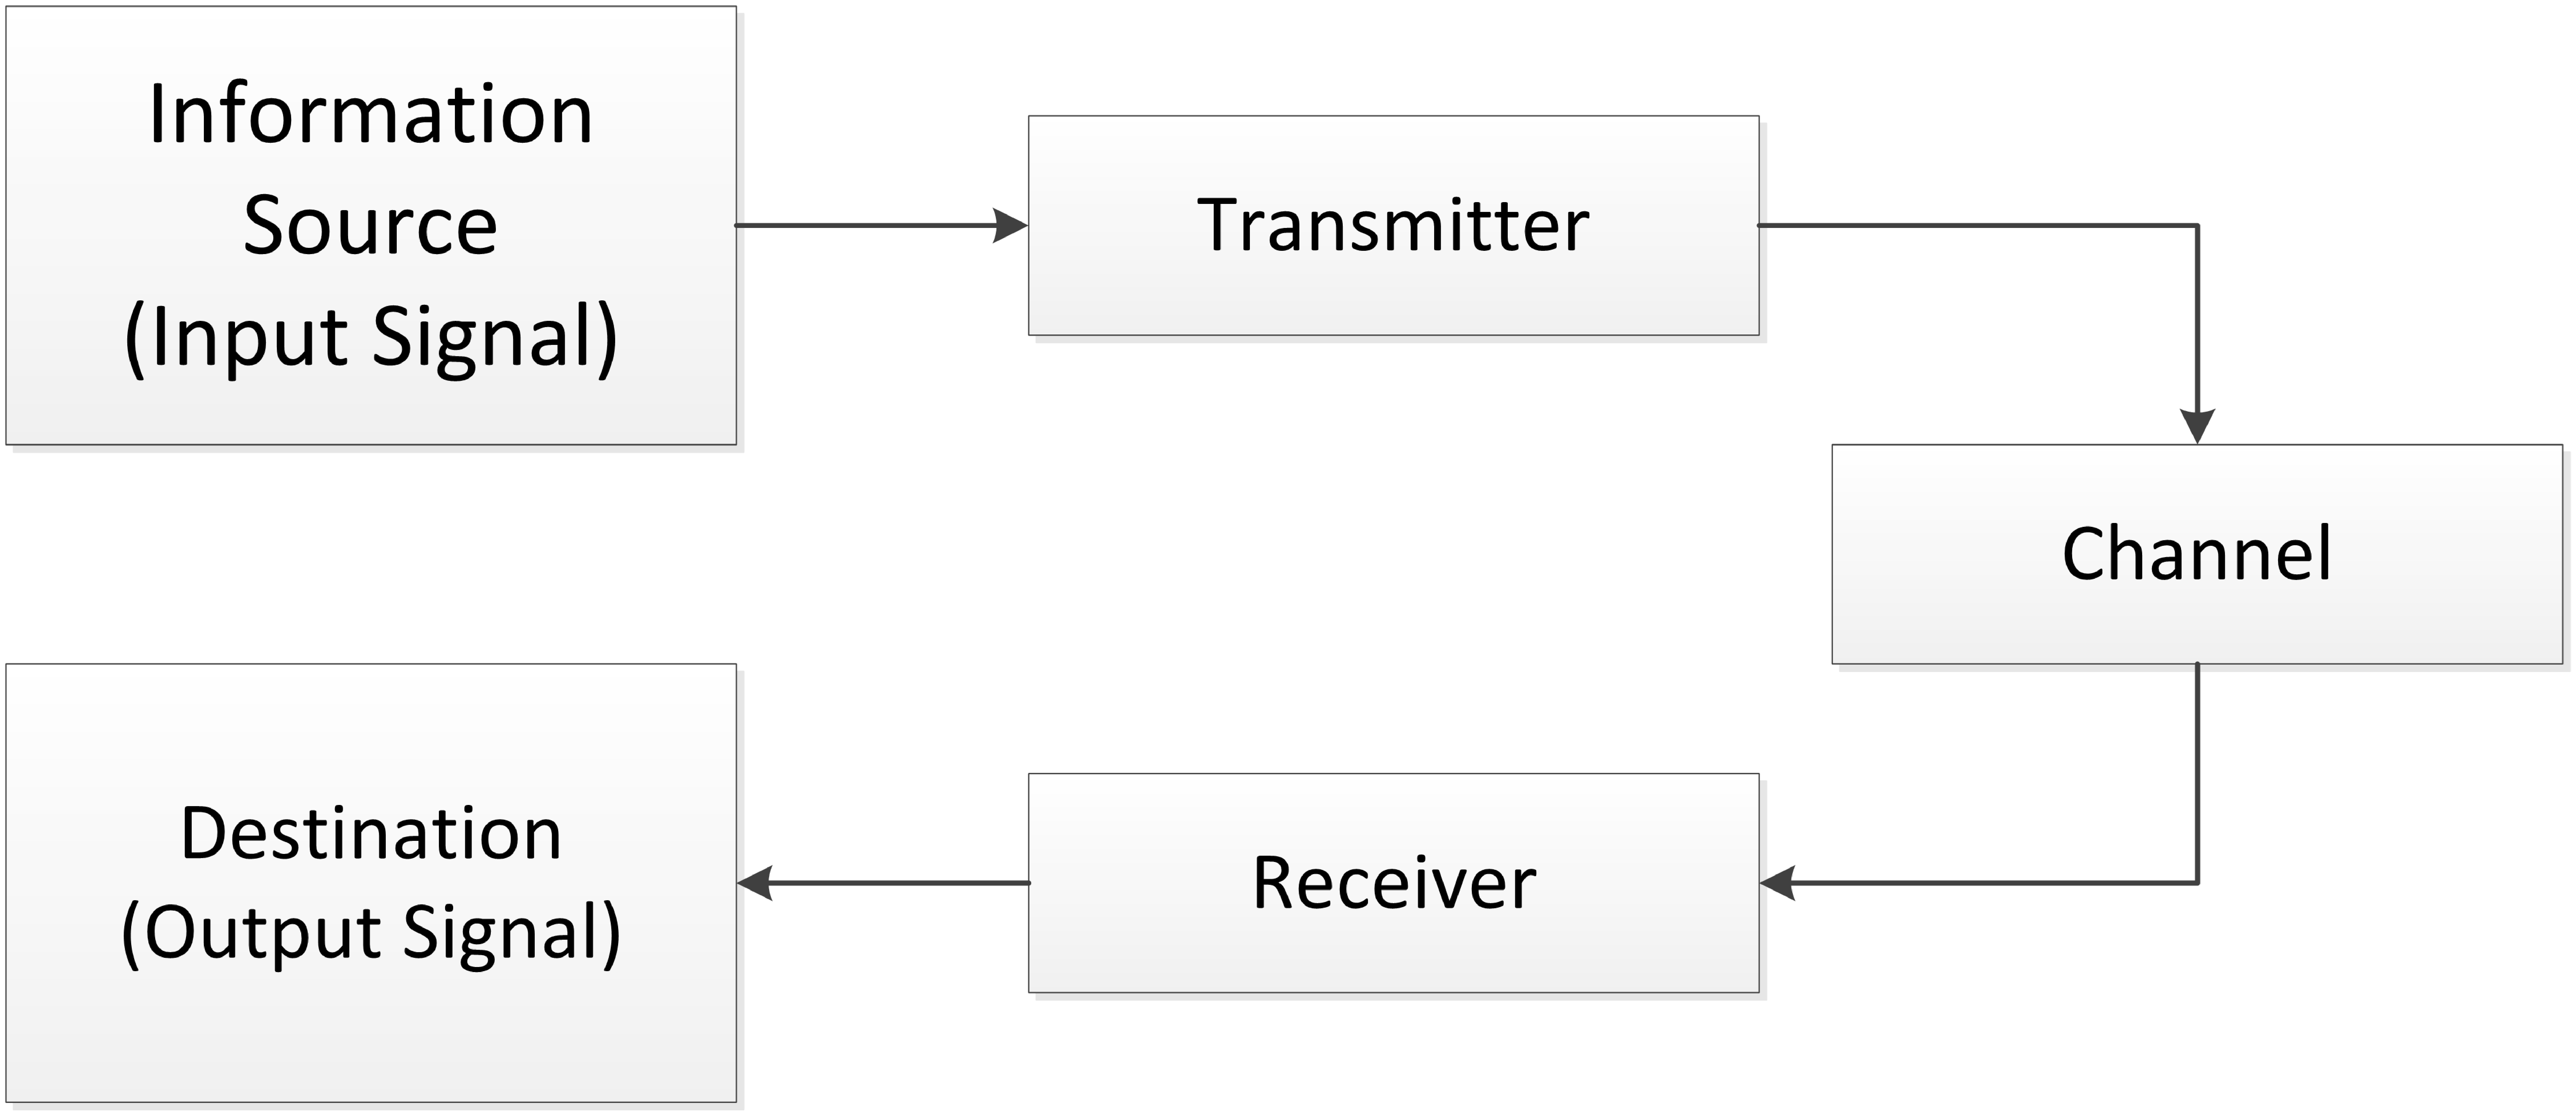
\includegraphics[width=0.65\textwidth]{./figures/digicom_simple}
    \caption{ A simple digital communication system block diagram.
    \label{fig:digicomsimple}}
\end{figure}

The transmitter is located at one point in space, the receiver is located at
some other point separate from the transmitter, and the channel is the medium
that provides the electrical connection between them. The former (transmitter),
in particular, is designed aiming to produce waveforms suitable for transmission
over the channel, a waveform. In the receiver the signal is normally corrupted
version of the transmitted signal, which is due to channel imperfections, noise
and interference. The receiver is designed to reconstruct a recognizable form of
the original message signal and to deliver it to a destination.

\subsection{Elements of Digital Communications Systems}

%block diagram of a digital communication system
\begin{figure}[htbp]
    \centering
    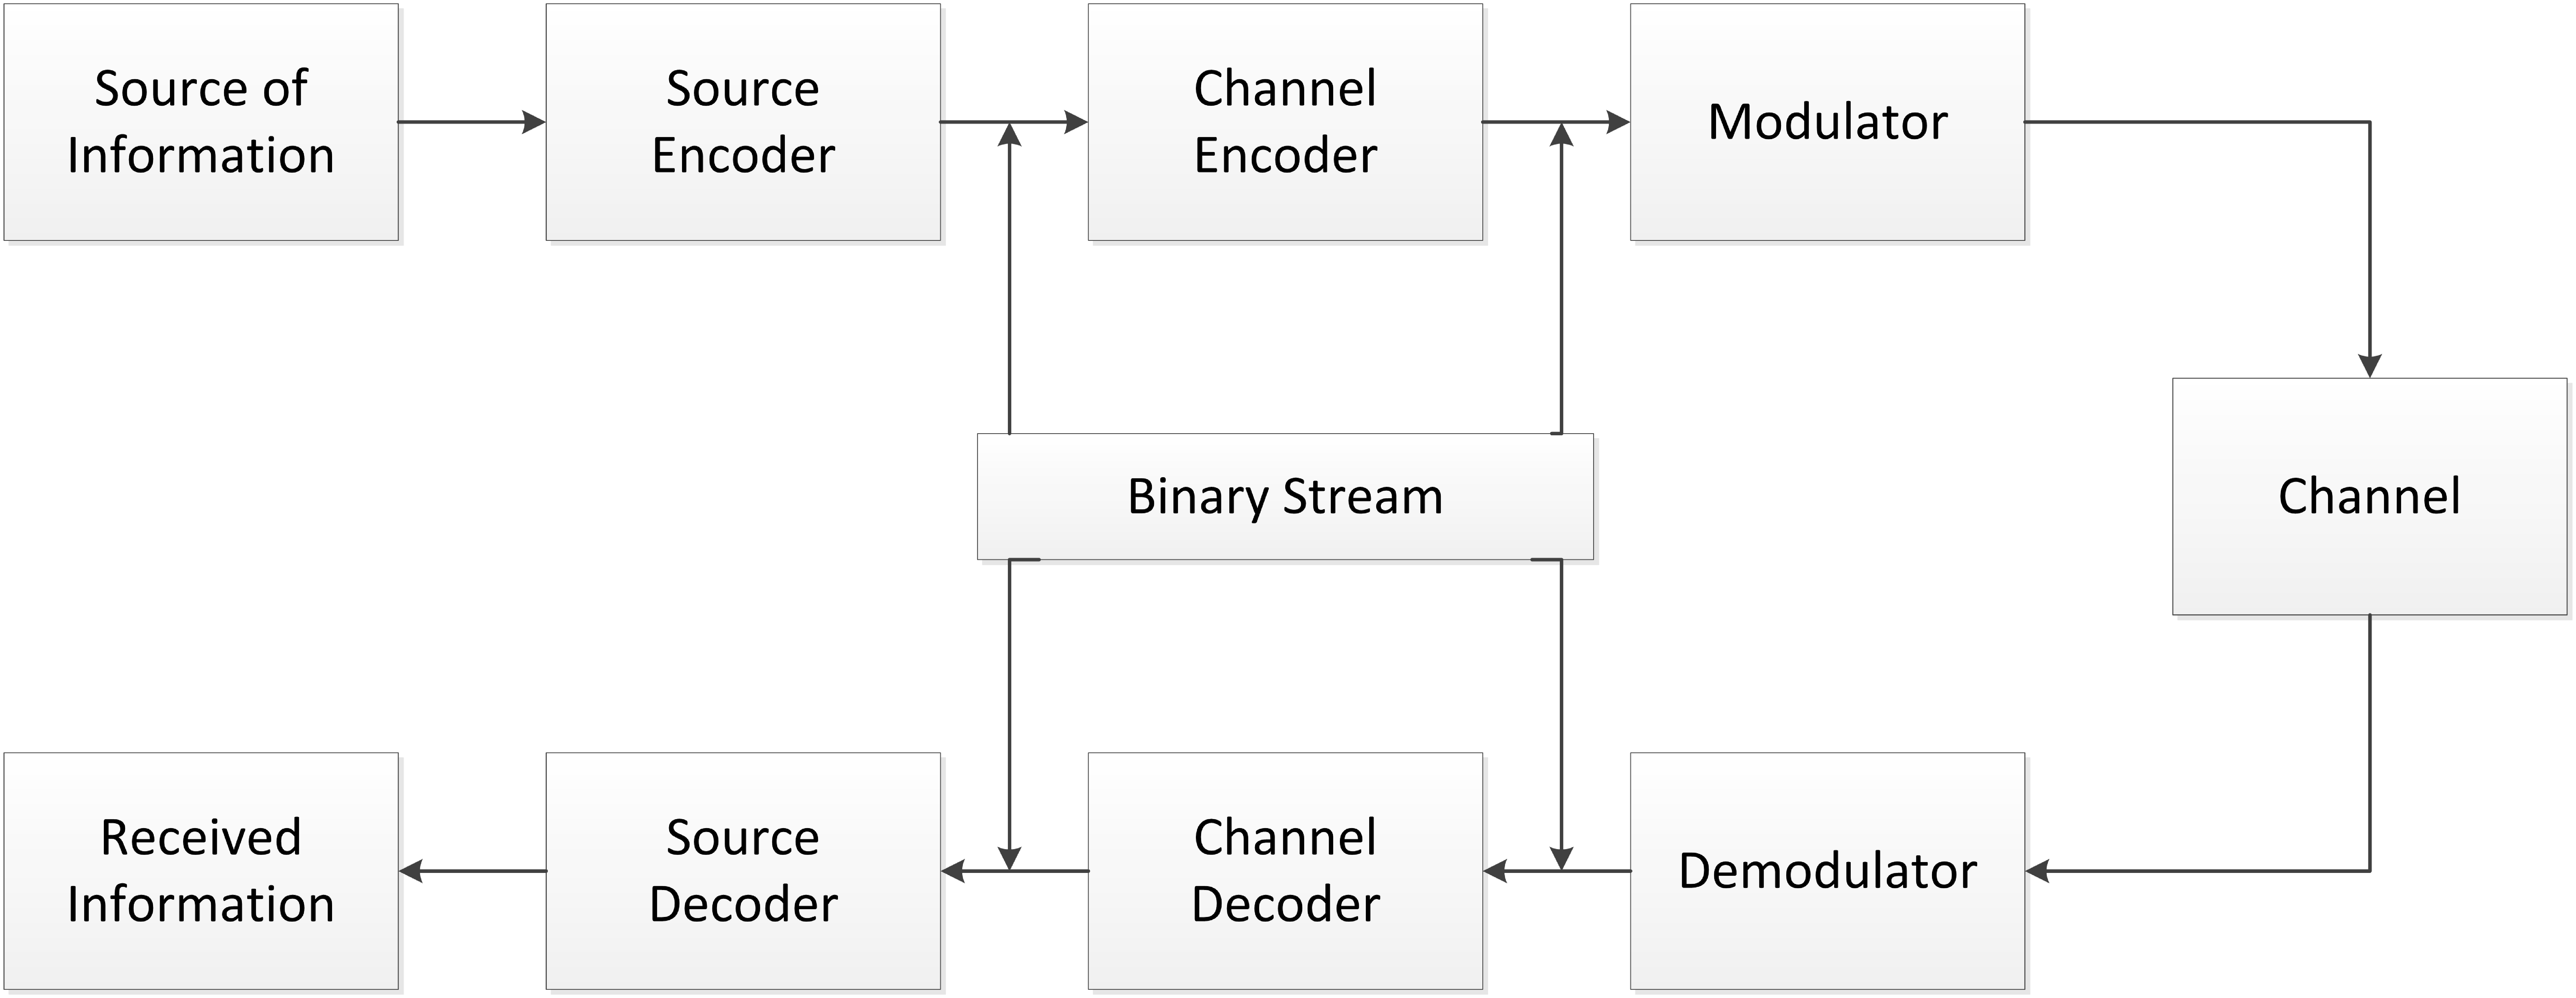
\includegraphics[width=0.85\textwidth]{./figures/digicom_bd}
    \caption{ Digital communication system block diagram.
    \label{fig:digcombd}}
\end{figure}

\subsubsection{Source of information}

The sources of information can be of two main kinds, \emph{analog information
sources} and \emph{digital information sources}. Analog information sources can
be human like voice, or natural like a humming bird. However, since Digital
communication systems work with a discrete and finite alphabet of symbols such
signals have to be converted to digital information prior to any process. Any
device that can record images or voice from the real world and can reproduce
back is making such analog to digital an digital to analog conversions
respectively.

Digital information sources are basically any information that was not
recorded or generated in the real world, it was generated by a software in a
PC. For example a digital painting or a 3D model.

\subsubsection{Source Encoder / Decoder}

The \emph{source encoder}  and \emph{source coder} converts the input symbol
sequence into a binary sequence (0 and 1) by assigning codewords to the symbols
in the input sequence. Basically the source encoder input is a analog waveform
and it samples, quantize and compress this analog waveform to a binary message
\cite{ocw:digicomm}.

At the receiver, the \emph{source decoder} converts the binary output of the
channel decoder into a analog waveform, doing the opposite operations of the
\emph{source encoder}. The decoder for a system using fixed length code words is
quite simple, but the decoder for a system using variable length code words can
be very complex \cite{ocw:digicomm}.

Aim of the source coding is to remove the redundancy in the transmitting
information, so that bandwidth required for transmission is minimized. This
approach is based on the probability of the symbol codeword is assigned. The
higher the probability, the shorter the codeword.

\subsubsection{Channel Encoder / Decoder}

Error control is accomplished by the channel coding operation that consists of
systematical addition of extra bits to the output of the source coder. These
extra bits do not convey any information but helps the receiver to detect and/or
correct some of the errors in the information bearing bits. There are two
methods of channel coding, the \textit{Block Coding} and \textit{Convolution
Coding}.

In the block coding method the encoder takes a block of ‘k’ information bits
from the source encoder and adds ‘r’ error control bits, where ‘r’ can be chosen
based on ‘k’ and error control capabilities desired, this process is
accomplished by a matrix multiplication and that is the origin of the "block" in
block coding. In the convolution coding process the message goes through a
sequence of tapped-delay line operations which works in the same way as
convolving the message with the impulse response of the code, with modulo-2
operations.

The Channel decoder recovers the information bits from the coded binary stream,
error detection and possible correction is also performed by the channel
decoder.

\subsubsection{Modulator}

The modulator converts the input bit stream into a waveform suitable for
transmission over the communication channel. Advanced modulation schemes such as
Orthogonal Frequency Division Multiplexing (OFDM) can be effectively used to
minimize the effects of channel noise to match the frequency spectrum of
transmitted signal with channel characteristics.

\subsubsection{Demodulator}

The extraction of the message from the information bearing waveform produced by
the modulation is accomplished by the demodulator. The output of the demodulator
are symbols which can be detected and the converted to bits to form a received
message.

\subsubsection{Channel}

The Channel is the medium of wave propagation (wireless in this work) then
creating a "connection" between transmitter and receiver. The different channels
are: pair of wires, coaxial cable, optical fiber, radio channel, satellite
channel or combination of any of these.

\subsection{Additional Modules}

%augmented block diagram
\begin{figure}[htbp]
    \centering
    
\includegraphics[width=0.85\textwidth]{./figures/digicom_plus}
    \caption{ Digital communication system block diagram with additional blocks.
    \label{fig:digicomplus}}
\end{figure}

Some additional blocks as shown in the block diagram  at Figure \ref{fig:digicomplus}
are used in most of digital communication system:

\begin{itemize}

  %\item \textbf{Encryptor:} Encryptor prevents unauthorized users from
    %understanding the messages and from injecting false messages into the system.

  \item \textbf{Multiplexer:} Multiplexer is used for combining signals from
different sources so that they share a portion of the communication system.

  \item \textbf{Demultiplexer:} DeMultiplexer is used for separating the different
signals so that they reach their respective destinations.

  %\item \textbf{Decryptor:} It does the reverse operation of that of the Encryptor.

\end{itemize}

\subsection{Synchronization}

Synchronization involves the estimation of both time and frequency. Coherent
systems need to synchronize their frequency reference with carrier in both
frequency and phase (carrier recovery). The synchronization begins with the
Automatic Gain Control (AGC) which scales the received waveform to a know power
level, then the timing recovery or carrier recovery process can be executed.

Timing or symbol recovery is the process of by with the receiver estimates the
symbol frequency of the received waveform, that process results in the best time
instants to sample a received waveform. Timing recovery is a requirement of all
digital communication systems \cite{akbook}.

Carrier recovery is a processes used in both coherent and non-coherent
demodulation where the phase and the frequency of the transmitter carrier wave
are recovered by the receiver and thus after having such information it is
possible to extract the information in the transmitted signal. Considering that
the phase and frequency of the transmitted wave probably will be affected by
noise, it is not a straight-forward method, it includes filtering and usually
feedback systems (PLLs) to correct the errors in phase or frequency caused by
the noise.

%-----------------------------------LTE-----------------------------------------

\section{Long Term Evolution} %OK
\label{let:lte}

\subsection{Overview}

Long Term Evolution (LTE) is a standard for wireless communication for
high-speed mobile devices and data terminals. LTE was first introduced in 3GPP
Release 8. It uses orthogonal frequency division multiplexing (OFDM) as its
radio access technology, together with advanced antenna technologies.

In addition to LTE, 3GPP also defined an IP-based, flat core network
architecture. This architecture was defined as part of the System Architecture
Evolution (SAE) effort specifying the Evolved Packet Core (EPC) network. The
LTE-SAE architecture and concepts have been designed for efficient support of
mass-market usage of any IP-based service. The architecture is based on an
evolution of the existing GSM/WCDMA core network.%, with simplified operations
%and smooth, cost-efficient deployment.

Moreover, work has also been done by 3GPP in cooperation with 3GPP2 (the CDMA
standardization body) to optimize interworking between CDMA and LTE-SAE. This means
that both CDMA and GSM operators can use the same standard with minor modifications
and thus making the deployment and roaming costs smaller.

The 3GPP radio access technology was developed towards and reduce cost per bit
implicating a lower cost and more variated services with a better user
experience. It was also thought in the flexibility of the existing and new
frequency  bands, giving LTE an scalable bandwidth (20MHz, 15MHz, 10MHz, 5MHz,
3MHz and 1.4MHz). Another noteworthy point is that the architecture and open
interfaces are simplified.

\subsection{Orthogonal Frequency-division Multiplexing Radio Technology} %+/-ok

LTE uses OFDM for the downlink (from the base station to the terminal or UE).
OFDM meets the LTE requirement for spectrum flexibility and enables
cost-efficient solutions for very wide carriers with high peak rates. It is a
well-established modulation scheme: for example, adopted in standards IEEE
802.11a/b/g, 802.16, HIPERLAN-2, DVB and DAB.

A representation of an OFDM signal can be seen in Figure \ref{fig:ofdmfreq}. In
this figure, a signal with 5 MHz bandwidth is shown, but the principle is of
course the same for the other Evolved UMTS Terrestrial Radio Access (E-UTRA)
bandwidths. Data symbols are independently modulated and transmitted over a high
number of closely spaced orthogonal subcarriers.

%ofdm scheme
\begin{figure}[htbp]
    \centering
    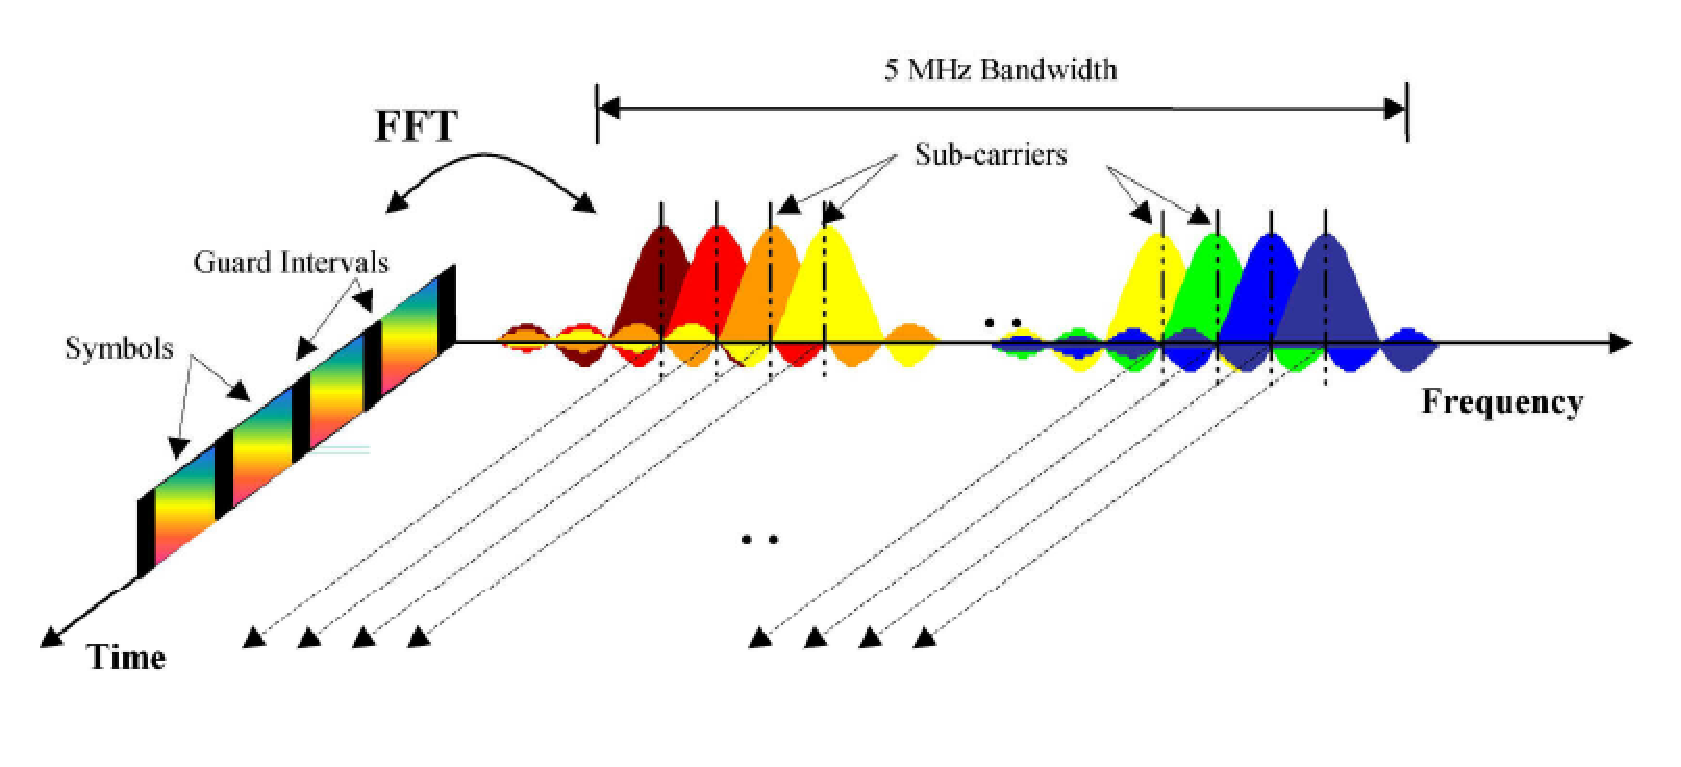
\includegraphics[width=0.65\textwidth]{./figures/ofdm_frequency}
    \caption{ Frequency-time representation of OFDM signal.
    \label{fig:ofdmfreq}}
\end{figure}

OFDM uses a large number of sub-carriers for multi-carrier transmission. The
basic LTE downlink physical resource can be seen as a time-frequency grid. In
the frequency domain, the spacing between the sub-carriers is 15 kHz. In
addition, the OFDM symbol duration time is $\frac{1}{\Delta f} + \text{cyclic
prefix duration}$. The cyclic prefix is used to maintain orthogonality between
the sub-carriers even for a time-dispersive radio channel.

The OFDM symbols are grouped into resource blocks. The resource blocks have a
total size of 180 kHz in the frequency domain and 0.5ms in the time domain. Each
user is allocated a number of so-called resource blocks in the time-frequency
grid and inside a resource block there are 12 subcarriers. The more resource
blocks a user gets, and the higher the modulation used in the resource element,
the higher the bit rate. Which resource blocks the user gets at a given point in
time, and how many, depends on advanced scheduling mechanisms in the frequency
and time dimensions. One resource element carries QPSK, 16QAM or 64QAM. With
64QAM, each resource element carries six bits.

In the uplink, LTE uses a pre-coded version of OFDM called single carrier
frequency division multiple access (SC-FDMA). This is to compensate for a
drawback with normal OFDM, which has a very high peak to average power ratio
(PAPR). High PAPR requires expensive and inefficient power amplifiers with high
linearity requirements, which increases the cost of the terminal and drains the
battery faster \cite{introlte}, \cite{umtslte}.

SC-FDMA solves this problem by grouping together the resource blocks in such a
way that it reduces the PAPR. Thus, it avoids the need for wider linear
operation bands of the power amplifier and also power consumption. A low PAPR
also improves coverage and cell-edge performance \cite{introlte}.

Since this work shall focus on the radio frontend part of the system, implementing
a downlink scheme, it is interesting to dwell more in the LTE downlink and uplink
schemes.

\subsection{Downlink Scheme}%OK

The downlink transmission scheme for E-UTRA FDD and TDD modes is based on
conventional OFDM. In an OFDM system, the available spectrum is divided into
multiple carriers, called subcarriers as explained in the previous subsection.
Each of these subcarriers is independently modulated by a a low rate data
stream, which allows robustness against multipath fading and efficient
equalization schemes.

The user data is carried on the Physical Downlink Shared Channel (PDSCH). The
PDSCH is the only channel that can be QPSK, 16QAM or 64QAM modulated. The
Downlink channel schematic can be seen in Figure \ref{fig:dlchann} with channels
delay spread. The delay spread is the time between the symbol arriving on the
first multi-path signal and the last multi-path signal component, typically
several $\mu s$ dependent on the environment (i.e. indoor, rural, suburban, city
center). The guard interval has to be selected in that way, that it is greater
than the maximum expected delay spread. In E-UTRA, the guard interval is a
cyclic prefix which is inserted prior to each OFDM symbol.

In practice, the OFDM signal can be generated using \textit{IFFT} (Inverse Fast
Fourier Transform) operation. The \textit{IFFT} converts a number N of complex
data symbols used in the frequency domain bins into the time domain signal. Such
an N-point \textit{IFFT} is illustrated in Figure \ref{fig:ofdmsymbol} where
$a(mN+n)$ refers to the nth subcarrier modulated data symbol, during the time
period $mT_u < t \le (m+1)T_u$ \cite{umtslte}.

%ofdm symbols
\begin{figure}[htbp]
    \centering
    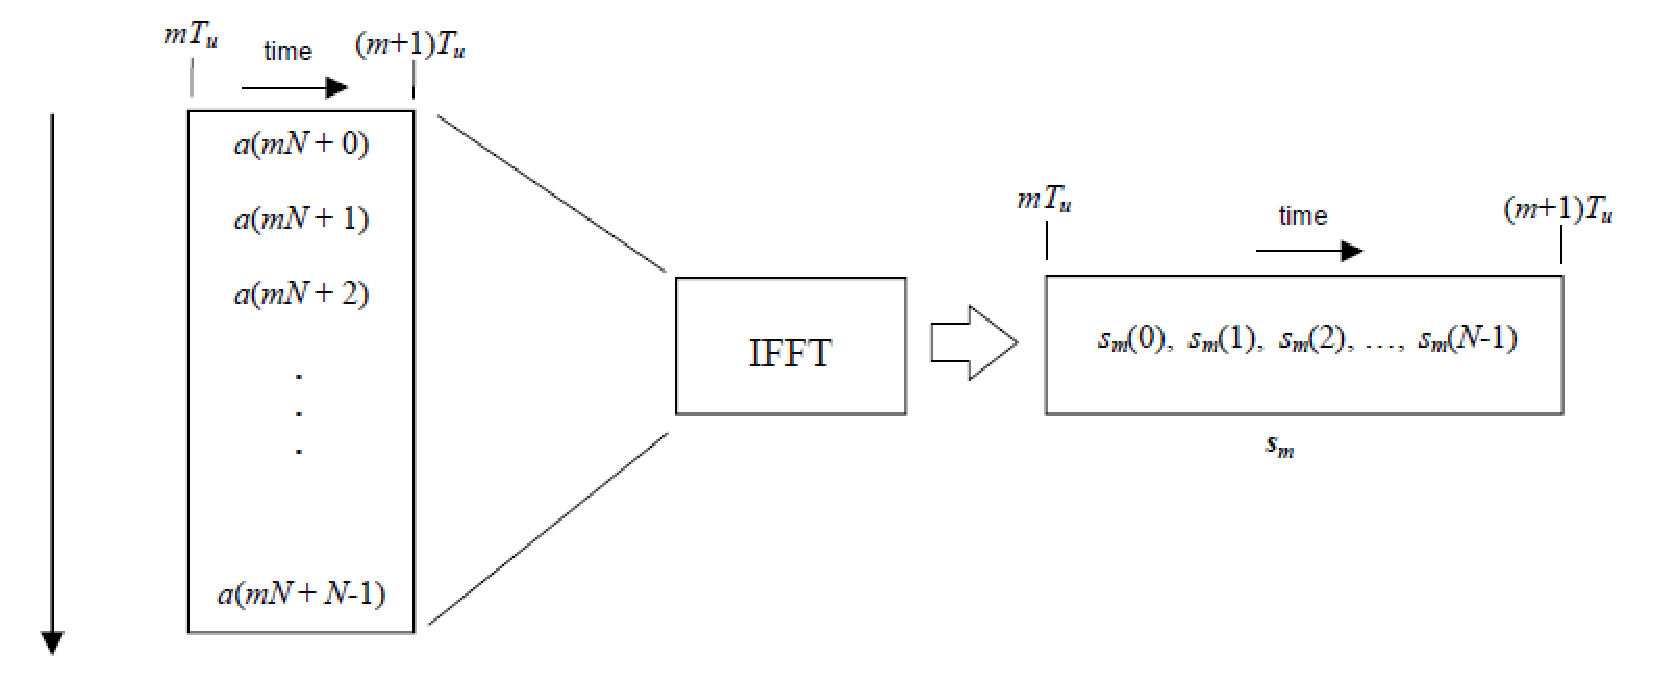
\includegraphics[width=0.65\textwidth]{./figures/ofdm_symbol_gen}
    \caption{ OFDM symbol generation \cite{umtslte}.
    \label{fig:ofdmsymbol}}
\end{figure}

The vector $sm$ is defined as the \emph{time-domain OFDM symbol}. It is the time
superposition of the $N$ narrowband modulated sub-carriers. Therefore, from a
parallel stream of $N$ sources of data, each one independently modulated, a
waveform composed of N orthogonal sub-carriers is obtained. Figure
\ref{fig:ofdmchain} illustrates the mapping from a serial stream of QAM symbols
to N parallel streams, used as frequency domain bins for the \textit{IFFT}. The
N-point time domain blocks obtained from the \textit{IFFT} are then serialized
to create a time domain signal.

%ofdm signal chain
\begin{figure}[htbp]
    \centering
    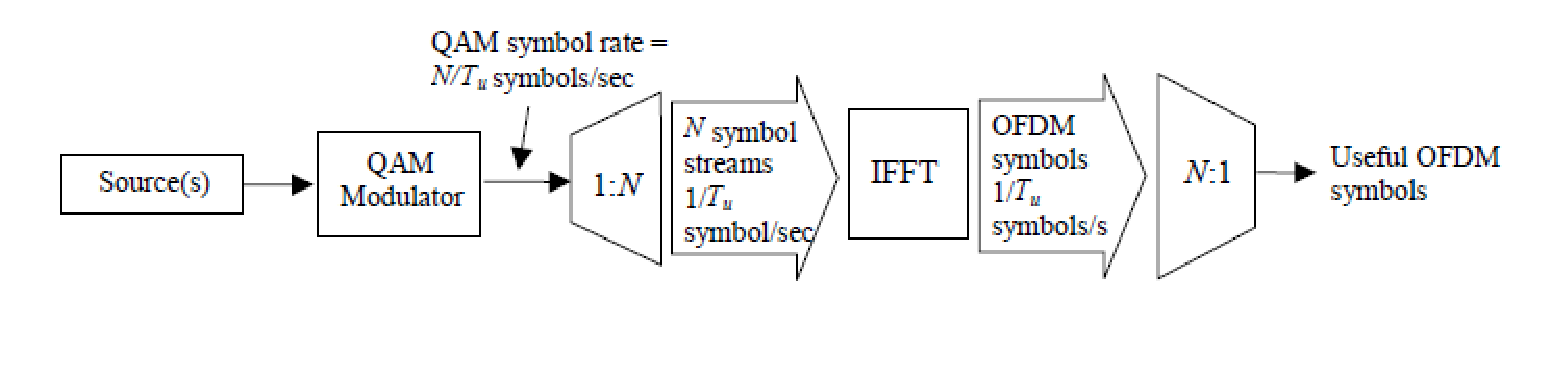
\includegraphics[width=0.65\textwidth]{./figures/ofdm_signal_chain}
    \caption{ OFDM signal generation \cite{umtslte}.
    \label{fig:ofdmchain}}
\end{figure}

In contrast to an OFDM transmission scheme, \textit{OFDM}A allows the access of
multiple users on the available bandwidth. Each user is assigned a specific
time-frequency resource. The data is allocated to a device (User Equipment, UE)
in terms of resource blocks, this means that one UE can be allocated integer
multiples of one resource block, whose representation can be seen in Figure
\ref{fig:ofdmresblk}. These resource blocks do not have to be adjacent to each
other. In the time domain, the scheduling decision can be modified every
transmission time interval of 1 ms corresponding to LTE sub-frame. All scheduling
decisions for downlink and uplink are done in the base station (enhanced NodeB,
eNodeB or eNB). The scheduling algorithm has to take into account the radio link
quality situation of different users, the overall interference situation,
Quality of Service requirements, service priorities, etc. and is a
vendor-specific implementation.

%ofdm resource block
\begin{figure}[htbp]
    \centering
    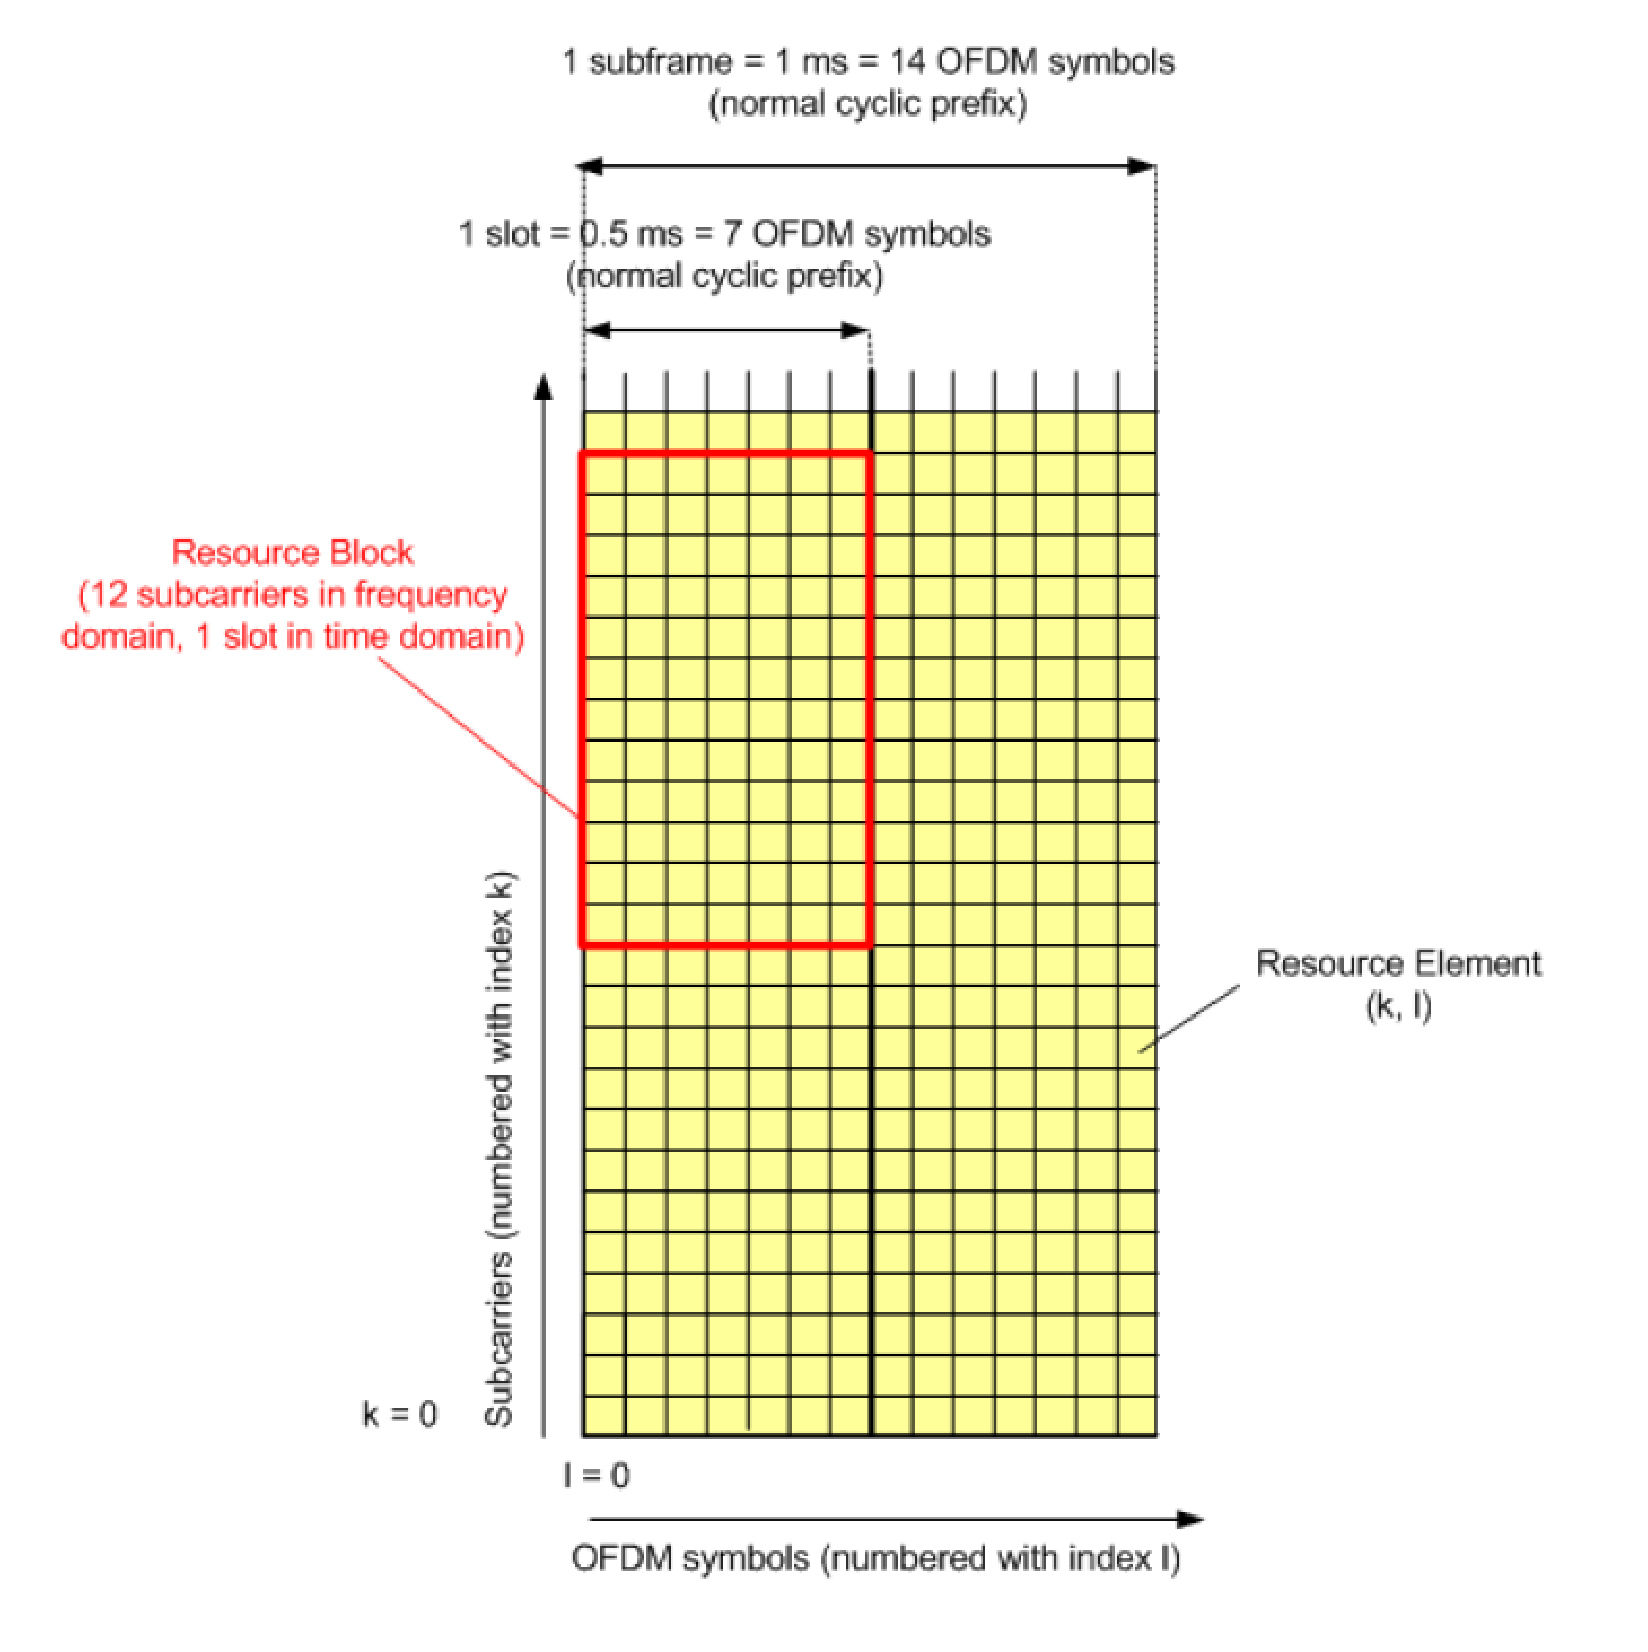
\includegraphics[width=0.65\textwidth]{./figures/ofdm_resource_block}
    \caption{ Resource block organization example \cite{umtslte}.
    \label{fig:ofdmresblk}}
\end{figure}

%downlink channel figura
\begin{figure}[htbp]
    \centering
    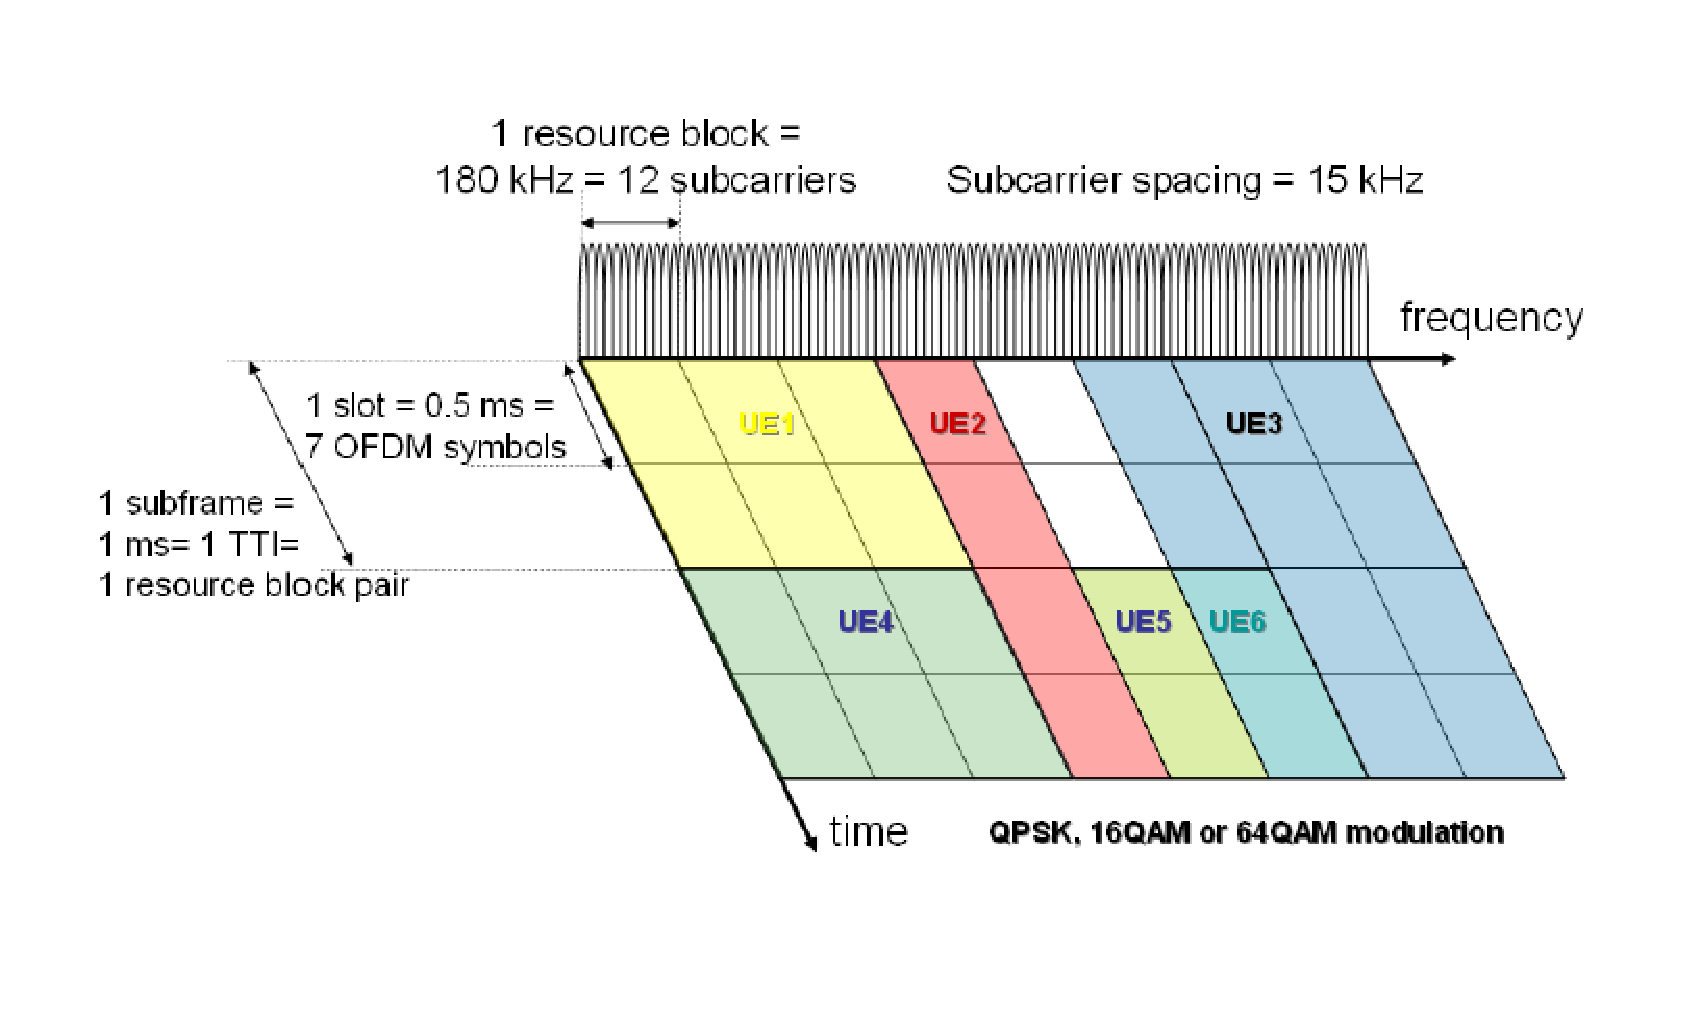
\includegraphics[width=0.70\textwidth]{./figures/downlink_channels}
    \caption{ OFDMA time-frequency multiplexing.
    \label{fig:dlchann}}
\end{figure}


\subsection{Uplink Scheme}%ok

During the study item phase of LTE, alternatives for the optimum uplink
transmission scheme were investigated \cite{umtslte}. While \textit{OFDMA} is
seen optimum to fulfill the LTE requirements in downlink, \textit{OFDMA}
properties are less favorable for the uplink. This is mainly due to unfavorable
PAPR properties of an \textit{OFDMA} signal, resulting in worse uplink coverage
and challenges in power amplifier design for battery operated handset, as it
requires expensive power amplifiers.

Thus, the LTE uplink transmission scheme for FDD and TDD mode is based on SC-
FDMA with cyclic prefix. Still, SC-FDMA signal processing has some similarities
with \textit{OFDMA} signal processing, so parameterization of downlink and
uplink can be harmonized.

There are different possibilities for generating an SC-FDMA signal. DFT-spread-
\textit{OFDM} \textit{(DFT-s-OFDM)} has been selected for E-UTRA. For
DFT-s-OFDM, a size-M DFT is first applied to a block of M modulation symbols,
prior to the IFFT. Then, QPSK, 16QAM and 64QAM are used as uplink E-UTRA
modulation schemes, the latter being optional for the UE. The DFT transforms the
modulation symbols into the frequency domain. The result is mapped onto the
available number of subcarriers. For LTE Release 8 uplink, only localized
transmission on consecutive subcarriers is allowed. An N-point \textit{IFFT}
where $N>M$ is then performed as in OFDM, followed by addition of the cyclic
prefix and parallel to serial conversion. The complete uplink scheme can be
illustrated by the diagram in Figure \ref{fig:uplinkbd}.

%figura uplink
\begin{figure}[htbp]
    \centering
    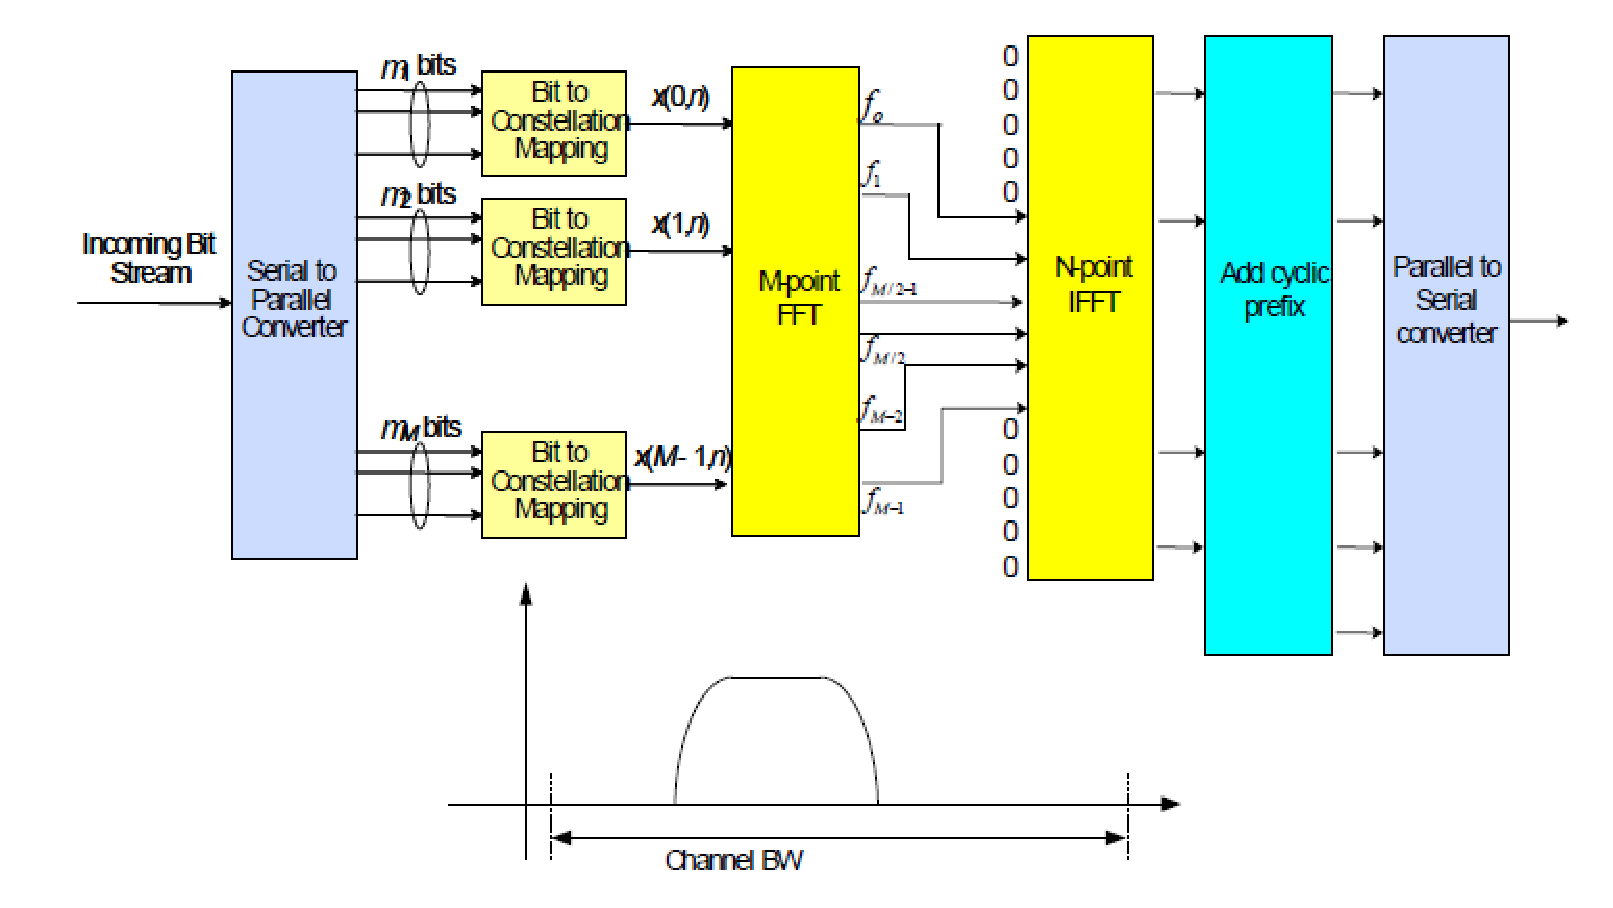
\includegraphics[width=0.65\textwidth]{./figures/uplink_scheme}
    \caption{ LTE uplink block diagram of DFT-s-OFDM.
    \label{fig:uplinkbd}}
\end{figure}
